\chapter{Synthetic Regulatory Networks} 

\section{Re-programming {\em E. coli}}

% how we program it (plasmids, etc)

\subsection{Basic Genetic Engineering}

A nice feature of {\em E. coli}, and other organisms as well, is that
an {\em E. coli} cell may contain one or more pieces of small,
circular {\em plasmid} DNA. These independently replicating pieces of
DNA are processed inside the cell much the same way as is genomic
DNA. Furthermore, it turns out to be fairly easy to construct
synthetic plasmids and stick them inside appropriately prepared
cells. Once there, the ...

\subsection{How we See What's Going On}

how we see what is going on: fluorescence, micrsoscopy, gene arrays,
RT-pcr, flow-cytometry, etc. 

Regulation: Transcription factors, ribozymes and other mechanisms

Observables: GFP, FRET, populations, single cells

\subsection{Inducing and Tuning Behaviors}

Inputs: IPTG, UV, periodic inputs, etc.


\section{Switches and Oscillators}

As discussed in Chapter~\ref{ch:in_vivo}, we can hook up genes that
produce transcription factors to each other. Consider a set of genes
$g_1$, ..., $g_n$. Draw each gene as a circle. If a gene produces a
transcription factor that activates or represses another gene, we
write an arrow or a line with a bar respectively from one gene to the
other. If a small molecule, called an {\em inducer}, activates or
deactivates a transcription factor, we draw similar arrows from nodes
representing the molecule to the arrow representing an
interaction as shown in Figure~\ref{fig:grn}. 

Synthetic biologists have built such networks by borrowing
transcription factors and promotors the regulatory regions from
various organisms. We describe some of these efforts below.

\subsection{The Bistable Switch}

In 2000, researchers from James Collins' lab published one of the
first artificial genetic regulatory networks designed specifically to
demonstrate the computational or information processing potential of
genetic regulatory networks. The system was a bi-stable switch
\cite{collins-toggle} designed from a pair of repressors that each
repressed the expression of the other, as shown in
Figure~\ref{fig:toggle}. The transcription factors used in the paper
are the lactose inhibitor {\em lacI} from {\em E. coli} for the first
repressor, and either tetracycline resistance {\em tetR} or $\lambda$
from the bacteriophage $\lambda$ for the second. As discussed above,
{\em lacI} can be induced by IPTG. $tetR$ can be induced by
anhydrotetracycline, a derivative of tetracycline. Finally, $\lambda$
can be induced by heat. The inducers allow experimentors to switch the
toggle switch from one state to the other.

\begin{figure}
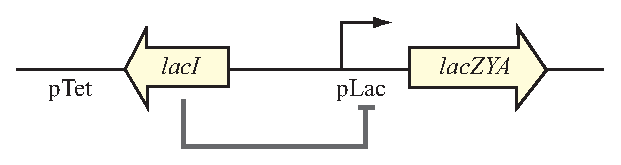
\epsfig{file=figures/toggle.eps, scale=0.8}
  \caption{\label{fig:toggle} The genetic toggle switch. Two
    repressors and their promotors are encoded on a plasmid. The first
    repressor is {\em lacI}, which acts on the pLac promoter. The pLac
    promoter is placed before the gene for the second repressor, which
    was either {\em tetR} or $\lambda$, and {\em gfp}. {\em tetR} acts
    on the pTet promoter, which is placed before {\em lacI}.}
\end{figure}

In the paper on the toggle switch, the authors propose the following
model
%
\begin{eqnarray}
X_1 & = & \frac{\alpha_1}{1+X_2^n} - X_1 \nonumber \\
X_2 & = & \frac{\alpha_2}{1+X_1^n} - X_2 . \label{eqn:bistable}
\end{eqnarray}
%
The authors note that bistability arises when the cooperativity
exceeds unity: $n,m>1$. For simplicity we assume that
$\alpha_1=\alpha_2=\alpha>0$.

\paragraph{The case when $n=m=1$:} When $n=1$, there is only on positive
equilibrium at
%
$$
X_1^* = X_2^* = \frac{-1 + \sqrt{1+4\alpha}}{2}.
$$
%
The Jacobian at this point is 
%
$$
A = \left . \left (
\begin{array}{cc}
-1 & -\frac{\alpha}{(1+X_2)^2} \\
-\frac{\alpha}{(1+X_2)^2} & -1 
\end{array}
\right ) \right |_{X=X^*}= 
\left (
\begin{array}{cc}
-1 & -\frac{4\alpha}{(1+X_2\sqrt{1+4\alpha})^2} \\
-\frac{4\alpha}{(1+X_2\sqrt{1+4\alpha})^2} & -1 
\end{array}
\right ) .
$$
%
The eigenvalues of $A$ are real and negative. Thus the single
equilibrium is stable and the system does not describe a bistable switch!

\paragraph{The case when $n=m>1$:} In this case, it is difficult to
obtain a closed form solution for $X^*$. One way to proceed is to
analyze the phase portrait. To do this, we define the following notion.

\begin{definition}
Given a two-dimensional system of the form 
\begin{eqnarray*}
\dot x_1 & = & f_1(x_1,x_2) \\
\dot x_2 & = & f_2(x_1,x_2),
\end{eqnarray*}
the first {\em nulcline} is the curve obtained by setting
$f_1(x_1,x_2) = 0$, i.e. where the first state variable $x_i$ is not
changing. The second {\em nulcline} is obtained via
$f_2(x_1,x_2)=0$. Anywhere two nuclines intersect is an equilibrium
point.
\end{definition}

The nulclines for the bistable swtich with $n=2$ and $\alpha=6$ are
shown, with the vector field defined by Equation~\ref{eqn:bistable},
in Figure~\ref{fig:bistable-nulclines}. Note that the nulclines
intersect in three points. Examination of various regions in the plot
indicates which are stable and which are not. For example, above the
two nulcines, all vectors point inward. Below, they point
outward. Along the nulcline for $\dot X_1 = 0$ and between the
separatrix (the blue line) and the top equilibrium point, $\dot X_2 >
0$. Along the $\dot X_2=0$ line and between the separatrix and the top
equilibrium point, $\dot X_1<0$. From this we can conclude that the
top equilibrium is stable. Similar reasoning shows the bottom
equilibrium is stable as well. 

\begin{figure}
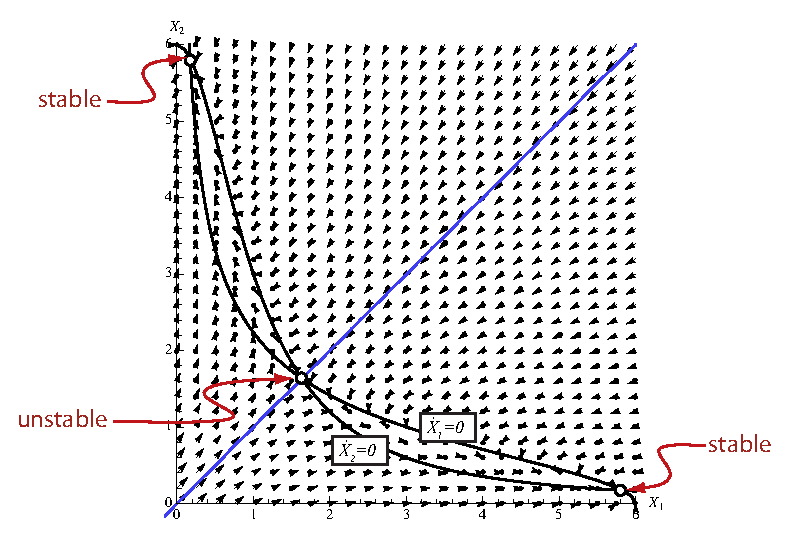
\epsfig{file=figures/bistable-nulclines.eps,scale=0.85}
\caption{\label{fig:bistable-nulclines} The nulclines and vector field
  associated with the bistable switch in Equation~\ref{eqn:bistable}
  with $n=2$ and $\alpha=6$. There are two stable equilibria and one
  unstable equilibrium.}
\end{figure}


\paragraph{No Cooperativity} There are papers stating that bistability
is in fact impossible with non-cooperative system
\cite{cherry-toggle}.  These papers use an extended Michaelis-Menton
somewhat blindly without recalling the assumptions that go into the
approximation. In particular, the assumption that there is a large
amount of $X_1$ cannot hold when there is a large amount of $X_2$. 

It turns out that a simple mass action model can produce bistability
without cooperativity. Consider the network
%
\begin{eqnarray*}
\varnothing \xrightharpoon[\text{}]{\text{$g_i \alpha_i$}} & X_i & 
            \xrightharpoon[\text{}]{\text{$\beta_i$}} \varnothing \\
g_1 + X_2 & \xrightleftharpoons[\text{$k_{-1}$}]{\text{$k_1$}} & g_{1,\mathit{off}} 
            \xrightharpoon[\text{}]{\text{$\gamma_1$}} g_1 \\
g_2 + X_1 & \xrightleftharpoons[\text{$k_{-2}$}]{\text{$k_2$}} & g_{2,\mathit{off}} 
            \xrightharpoon[\text{}]{\text{$\gamma_2$}} g_2 .
\end{eqnarray*}
%
Note that we have modeled the degradation of $X_i$ in two places. One,
$X_i$ simply degrades. Two, $X_i$ when bound to $g_j$ to make
$g_{j,\mathit{off}}$ degrades, turning $g_{j,\mathit{off}}$ into
$g_j$. We add this to the model, because when there is very little
$X_i$, the degradation of even the small amount of it that is bound to
$g_j$ is significant. 

It can be shown that the equation $\dot v = A K(v)$ has four
equilibria and that parameters can be found so that one has
$X_1=X_2<0$ while the other three have $X_1>0$ and $X_2>0$. The three
positive equilibra consist of two stable and one unstable equilibrium,
similar to the cooperative version of bistability above. 

\subsection{The Repressilator}

A construction similar to the bistable switch, and indeed appearing in
the same issue of Nature in 2000, is the ring oscillator made out of
three repressors \cite{elowitz-repressilator}, aptly named the
{\em repressilator}.

\subsection{Hysteresis Based Oscillators}

Circadian rhythms are responsible for many phenomena, the most famous
of which is the 17-year cycle of certain North American cicadas. Sleep
cycles in humans are another. The repressilator is not a likely model
for circadian rhythms, mostly because it is very sensitive to noise. A
more frequently proposed model for the kind of structure that likely
generates such oscillations is the {\em hysteresis based oscillator}
% http://www.nature.com/nature/journal/v403/n6767/pdf/403267b0.pdf
\cite{barkai-leibler-circadian}, which was to some extent implemented in 
% http://linkinghub.elsevier.com/retrieve/pii/S0092867403003465
\cite{ninfa-oscillator}.

% http://biodynamics.ucsd.edu/publications.htm
\cite{hasty-oscillator}

\subsection{A Bandbass Filter}

\cite{weiss-communication}

\section{RNA Regulatory Mechanisms}

Lock and key, ribozymes, etc.
\cite{rna-synthetic-biology}

\setcounter{exercount}{0}

\section{Problems}

\begin{exercise}
  Look up the equations used in the paper about the Repressilator
  \cite{elowitz-repressilator} and simulate them. 
\end{exercise}

\begin{exercise}
  Look up the equations used in the paper about the hysteresis-based
  oscillator that uses {\em araC} and {\em lacI}
  \cite{hasty-oscillator} and simulate them.
\end{exercise}